\chapterauthor{Remigiusz Wojewódzki}
% \chapterauthor{Remigiusz Wojewódzki}
\chapter[Sąsiedztwo Motzkina \ldots]{Sąsiedztwo Motzkina dla Permutacyjnego Problemu Przepływowego}
\thispagestyle{empty}
\vspace{-8mm} {\large Remigiusz Wojewódzki} \vspace{8mm}

\section{Wstęp}

Permutacyjny problem przepływowy (Flow Shop Problem) polega na znalezieniu permutacji $n$ zadań wykonywanych na $m$ maszynach w tej samej kolejności, minimalizującej czas zakończenia (makespan) $C_{\max}$. Klasyczne sąsiedztwa (np. zamiana sąsiadujących elementów) eksplorują przestrzeń lokalnie i płytko. Motywacją tej pracy jest skonstruowanie bogatszego ruchu złożonego, który zachowuje strukturę umożliwiającą efektywną optymalizację, obejmując jednocześnie wiele skoordynowanych zmian. Obecny tekst jest poniekąd kontynuacją wcześniejszej pracy autora \cite{Fibona}, w której zaproponowano otoczenie nazwane otoczeniem \emph{Fibonacciego}. Jest to otoczenie, które wykonuje wiele zmian w jednym ruchu, lecz jedynie sąsiadujących wartości, bez możliwości przecięcia. W dalszej części rozdziału zostanie zaproponowane nowe otoczenie, bazujące na liczbach Motzkina.

\section{Flow Shop Problem}

Dla macierzy czasów przetwarzania \(P = [p_{k,j}]_{m \times n}\) (maszyna \(k=1,\dots,m\), zadanie \(j=1,\dots,n\)), permutacja \(\pi\) definiuje kolejność zadań. Permutacje i~ich zależności można analizować z użyciem dodatnio określonych funkcji na grupach permutacji, co daje teoretyczne podstawy badania korelacji między sekwencjami zadań \cite{Bozejko2015}. Niech \(C_{k,j}\) oznacza czas zakończenia zadania \(j\) (w~kolejności \(\pi\)) na maszynie \(k\), spełniający zależności:
\[
C_{1,j} = C_{1,j-1} + p_{1,\pi(j)},\quad
C_{k,1} = C_{k-1,1} + p_{k,\pi(1)},
\]
\begin{equation}\label{eq_c_kj}
C_{k,j} = \max\{C_{k,j-1},\, C_{k-1,j}\} + p_{k,\pi(j)}, \quad \text{dla } k=1,\dots,m,\; j=1,\dots,n.
\end{equation}
Maksum \(C_{\max} = C_{m,n}\) należy zminimalizować. Celem FSP jest znalezienie permutacji \(\pi\), która \emph{minimalizuje} \(C_{\max}\), tj. czas zakończenia ostatniego zadania na ostatniej maszynie przy przetwarzaniu w kolejności \(\pi\).

\section{Struktury sąsiedztw}
Za \cite{vanlaarhoven1992} \emph{sąsiedztwo} rozwiązania \(x\) to zbiór rozwiązań otrzymywanych poprzez dozwoloną modyfikację \(x\). Wyznacza ono sposób eksploracji i eksploatacji przestrzeni rozwiązań w trakcie poszukiwań.

Nawiązując do Ahuji i in. \cite{ahuja2002,glover1997}, można wskazać ogólne metody konstruowania bardzo dużych sąsiedztw (VLSN). Obejmują one generowanie nowych rozwiązań przez łączenie elementów z wielu rozwiązań odniesienia, co umożliwia eksplorację większych obszarów przestrzeni. Innym podejściem jest użycie programowania dynamicznego do przyspieszania obliczeń i efektywnego budowania sąsiedztw dla dużych danych. Kluczowym komponentem są grafy ulepszeń pozwalające szybko oceniać obiecujące ruchy. Metody VLSN są często integrowane z metaheurystykami (Tabu Search, Simulated Annealing), tworząc algorytmy iteracyjne, zdolne skutecznie poszukiwać rozwiązań wysokiej jakości.
\paragraph{Sąsiedztwo \emph{Fibonacciego}} Opisane w pracy \cite{Fibona} sąsiedztwo \emph{Fibonacciego} należy do grona bardziej złożonych. W obrębie pojedynczego ruchu zostaje wykonanych $n$ zamian sąsiadujących ze sobą elementów w celu minimalizacji $C_{\max}$ dla danej permutacji. Do obliczenia, które elementy mają zostać zmienione wykorzystane zostało programowanie dynamiczne pozwalające optymalizować ilość obliczeń.


\section{Charakterystyka Liczb Motzkina}

Liczby Motzkina $M_n$, bazując na \cite{Motzkin_numbers}, enumerują \emph{planarne} (nieprzecinające się) struktury nad zbiorem $n$ uporządkowanych punktów, gdzie każdy punkt może być (i) początkiem łuku, (ii) końcem łuku, lub (iii) izolowany. Stanowią one uogólnienie liczb Catalana -- podczas gdy te ostatnie wymagają pełnego sparowania, liczby Motzkina dopuszczają punkty pojedyncze.

\paragraph{Równoważne reprezentacje.}
Obiekty Motzkina można interpretować jako:
\begin{enumerate}
  \item Ścieżki kratowe z krokami $(1,+1)$, $(1,0)$, $(1,-1)$ nieopadające poniżej osi $y=0$.
  \item Nieprzecinające się rodziny łuków nad linią z opcjonalnymi izolowanymi punktami.
  \item Wzbogacone triangulacje lub podziały wielokątów.
\end{enumerate}
W naszym sąsiedztwie każdy indeks permutacji może uczestniczyć jako lewy koniec łuku, prawy koniec łuku lub pozostać nienaruszony -- dokładnie trzy stany odpowiadające strukturze Motzkina.

\paragraph{Rekurencje.}
Podstawowa rekurencja konwolucyjna wynika z rozkładu pierwszego punktu:
\begin{align*}
M_0 &= 1,\quad M_1 = 1,\\
M_n &= M_{n-1} + \sum_{k=0}^{n-2} M_k\, M_{n-2-k}\quad (n \ge 2).
\end{align*}
Interpretacja: jeśli punkt 0 jest izolowany, pozostaje $M_{n-1}$ konfiguracji; jeśli otwiera łuk zamykany w punkcie $k+1$, wnętrze (punkty $1\ldots k$) i zewnętrzny ogon (punkty $k+2\ldots n-1$) są niezależne, dając iloczyn $M_k M_{n-2-k}$.

Alternatywna rekurencja liniowa:
\[
M_n = \frac{(2n+1)M_{n-1} + 3(n-1)M_{n-2}}{n+2},\quad n \ge 2.
\]

Funkcja tworząca:
\[
M(x) = \sum_{n\ge0} M_n x^n = \frac{1 - x - \sqrt{1 - 2x - 3x^2}}{2x^2}.
\]

\paragraph{Asymptotyka}
Asymptotycznie $M_n \sim c\,3^n / n^{3/2}$ dla stałej $c = \frac{3\sqrt{3}}{2\sqrt{\pi}}$. Przestrzeń dopuszczalnych ruchów złożonych rośnie znacznie wolniej niż $2^{\binom{n}{2}}$ (zbiór wszystkich podzbiorów par indeksów), czyniąc pełne programowanie dynamiczne praktycznym.

\begin{table}[ht]
  \centering
  \caption{Pierwsze liczby Motzkina ($n=0..10$).}
  \begin{tabular}{@{}rcccccccccccc@{}}
    \toprule
    $n$ & 0 & 1 & 2 & 3 & 4 & 5 & 6 & 7 & 8 & 9 & 10 \\
    \midrule
    $M_n$ & 1 & 1 & 2 & 4 & 9 & 21 & 51 & 127 & 323 & 835 & 2188 \\
    \bottomrule
  \end{tabular}
\end{table}

\paragraph{Przykład: obliczanie $M_4$.}
Stosując rekurencję konwolucyjną:
\[
\begin{aligned}
M_2 &= M_1 + M_0 M_0 = 1 + 1 = 2, \\
M_3 &= M_2 + (M_0 M_1 + M_1 M_0) = 2 + 2 = 4, \\
M_4 &= M_3 + (M_0 M_2 + M_1 M_1 + M_2 M_0) = 4 + (2 + 1 + 2) = 9.
\end{aligned}
\]

\medskip
Mając ustalone kombinatoryczne podstawy liczb Motzkina, przechodzimy teraz do konstrukcji sąsiedztwa dla permutacyjnego problemu przepływowego.


\section{Struktura Sąsiedztwa Motzkina}

Proponowane sąsiedztwo reprezentuje przejście od klasycznych ruchów jednoparametrowych (np. pojedyncza zamiana sąsiadujących elementów) do \emph{strukturalnie złożonych} multi-ruchów, które mogą transformować permutację w jednym kroku poprzez kilka skoordynowanych lokalnych modyfikacji -- podobnie do Dynasearch lub sąsiedztwa Fibonacciego\cite{Fibona}.

Przewodnia idea polega na ograniczeniu eksplozji kombinatorycznej poprzez narzucenie ścisłej, łatwej do zweryfikowania struktury: każda para indeksów $(i,j)$ opisuje zamianę końców segmentu, a zbiór takich par jest dopuszczalny tylko wtedy, gdy odpowiadające łuki (interpretowane jako połączenia $i \to j$ nad linią indeksów) są \emph{nieprzecinające się}, mogą być \emph{zagnieżdżone}, ale nie dzielą końców. W ten sposób w jednej iteracji przeszukujemy szerszy horyzont potencjalnych rozwiązań, zachowując kontrolę złożoności.

\subsection{Definicja Ruchu i Warunki Dopuszczalności}
\paragraph{Zamiana końców.}
Dla permutacji $\pi = (\pi_0,\pi_1,\ldots,\pi_{n-1})$ i pary indeksów $(i,j)$ spełniającej $0 \le i < j < n$, definiujemy \emph{zamianę końców} jako operację:
\[
S_{i,j}(\pi) = (\pi_0,\ldots,\pi_{i-1},\; \pi_j,\; \pi_{i+1},\ldots,\pi_{j-1},\; \pi_i,\; \pi_{j+1},\ldots,\pi_{n-1}).
\]
Ta operacja zamienia wyłącznie elementy na pozycjach $i$ i $j$, zachowując kolejność wszystkich elementów pośrednich $\pi_{i+1},\ldots,\pi_{j-1}$. Lokalnie segment $[\pi_i,\pi_{i+1},\ldots,\pi_{j-1},\pi_j]$ przekształca się w $[\pi_j,\pi_{i+1},\ldots,\pi_{j-1},\pi_i]$.

\paragraph{Ruch złożony: zbiór współbieżnych zamian.}
\emph{Ruch złożony} jest zbiorem $\mathcal{M} = \{(i_1,j_1), (i_2,j_2), \ldots, (i_k,j_k)\}$ par indeksów. Zbiór $\mathcal{M}$ jest \emph{dopuszczalny}, jeśli spełnia następujące warunki:

\begin{enumerate}
  \item \textbf{Rozłączność końców}: Dla dowolnych dwóch par $(i_a,j_a), (i_b,j_b) \in \mathcal{M}$ mamy $\{i_a,j_a\} \cap \{i_b,j_b\} = \varnothing$ (żadne dwie pary nie dzielą indeksu).
  
  \item \textbf{Brak przecięć}: Wzór $i_a < i_b < j_a < j_b$ jest zabroniony dla dowolnych $(i_a,j_a), (i_b,j_b) \in \mathcal{M}$ (łuki nie mogą się przecinać).
  
  \item \textbf{Zagnieżdżanie dozwolone}: Konfiguracja $i_a < i_b < j_b < j_a$ jest akceptowalna (para wewnętrzna całkowicie zawarta w parze zewnętrznej).
\end{enumerate}

Zastosowanie wszystkich zamian ze zbioru $\mathcal{M}$ w kolejności rosnących lewych końców $i_k$ daje unikalny wynik -- warunki (1)–(3) gwarantują, że żadna para nie interferuje z efektem innej pary. Każda para modyfikuje tylko dwa elementy permutacji na pozycjach końcowych; wewnętrzny segment zachowuje kolejność, a symulacja zagnieżdżonych łuków przebiega niezależnie.
\begin{figure}[ht]
  \centering
  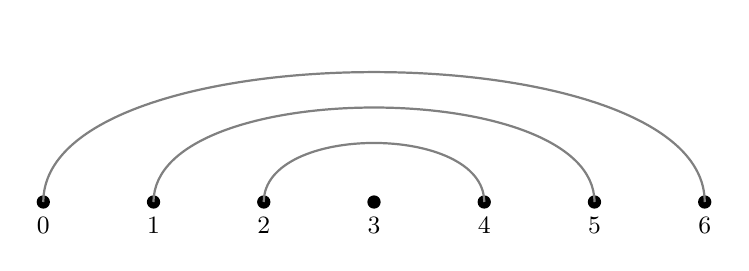
\begin{tikzpicture}[scale=1.0, baseline=(current bounding box.center)]
    \def\N{7}
    \def\DX{1.4}
    \def\Ybase{0}
    \foreach \i in {0,...,6} {
      \coordinate (P\i) at (\i*\DX,\Ybase);
      \fill (P\i) circle (2.4pt);
      \node[below=2pt, font=\small] at (P\i) {\i};
    }
    \draw[gray, thick] (P0) .. controls +(.0,2.2) and +(-.0,2.2) .. (P6);
    \draw[gray, thick] (P1) .. controls +(.0,1.6) and +(-.0,1.6) .. (P5);
    \draw[gray, thick] (P2) .. controls +(.0,1.0) and +(-.0,1.0) .. (P4);
  \end{tikzpicture}
  \caption{Przykład dopuszczalnego ruchu złożonego: zagnieżdżone łuki $(0,6)$, $(1,5)$, $(2,4)$; punkt 3 izolowany.}
\end{figure}

\paragraph{Bijekcja z obiektami Motzkina.}
Kluczowa obserwacja jest taka, że zbiór dopuszczalnych ruchów złożonych dla $n$ indeksów ma moc dokładnie równą $M_n$ (liczbie Motzkina). Interpretacja: każdy indeks $0 \le i < n$ może być w jednym z trzech stanów:
\begin{itemize}
  \item \textbf{Lewy koniec łuku}: istnieje para $(i,j) \in \mathcal{M}$.
  \item \textbf{Prawy koniec łuku}: istnieje para $(k,i) \in \mathcal{M}$.
  \item \textbf{Izolowany}: indeks nie uczestniczy w żadnej parze.
\end{itemize}
Ta właściwość trzech stanów odpowiada dokładnie definicji obiektów Motzkina (ścieżki z krokami $+1$, $0$, $-1$ lub rodziny łuków z izolowanymi punktami). Warunki (1)–(3) kodują nieprzecinanie się i rozłączność, co jest istotą struktury Motzkina.

\paragraph{Rozmiar przestrzeni i implikacje algorytmiczne.}
Przestrzeń dopuszczalnych ruchów złożonych ma rozmiar $M_n \sim c \cdot 3^n / n^{3/2}$, który jest znacznie mniejszy niż $2^{\binom{n}{2}}$ (wszystkie podzbiory par indeksów). Ten kontrolowany rozmiar przestrzeni uzasadnia użycie pełnego programowania dynamicznego do wyboru optymalnego ruchu złożonego -- w przeciwieństwie do naiwnego przeszukiwania wykładniczej liczby kombinacji, algorytm DP operuje na $O(n^2)$ stanach, rozważając $O(n)$ kandydatów na stan.


\section{Algorytm Wyboru Optymalnego Ruchu Złożonego}

Mając zdefiniowaną przestrzeń dopuszczalnych ruchów złożonych, potrzebujemy algorytmu, który w czasie wielomianowym wybiera zbiór par $\mathcal{M}$ minimalizujący makespan. Algorytm składa się z pięciu kroków:
\begin{enumerate}
  \item Obliczanie kolumn zakończenia prefiksów $F[k][r]$ (preprocessing).
  \item Enumeracja delt $\Delta_{i,j}$ dla wszystkich par $(i,j)$.
  \item Programowanie dynamiczne: wypełnianie tablicy $\mathrm{dp}[L][R]$.
  \item Rekonstrukcja wybranego zbioru par $\mathcal{M}$.
  \item Zastosowanie zamian do permutacji $\pi$.
\end{enumerate}

\paragraph{Obliczanie delt} Dla każdej pary indeksów $(i,j)$ z $0 \le i < j < n$ obliczamy zmianę makespan:
\[
\Delta_{i,j} = C_{\max}(S_{i,j}(\pi)) - C_{\max}(\pi).
\]

W implementacji używamy \emph{kolumn zakończenia prefiksów} $F[k][r]$, gdzie $F[k][r]$ oznacza czas zakończenia na maszynie $r$ po przetworzeniu pierwszych $k$ zadań permutacji $\pi$. Obliczamy te kolumny używając standardowego DP dla FSP:
\[
\begin{aligned}
F[0][r] &= 0 \quad \text{dla wszystkich } r, \\
F[k][0] &= F[k-1][0] + p_{0,\pi_{k-1}}, \\
F[k][r] &= \max(F[k][r-1], F[k-1][r]) + p_{r,\pi_{k-1}}, \quad r \ge 1,
\end{aligned}
\]
gdzie $p_{r,j}$ jest czasem przetwarzania zadania $j$ na maszynie $r$.

Następnie dla pary $(i,j)$, zaczynając od stanu prefiksu $F[i]$, symulujemy nową kolejność segmentu:
\[
[\pi_j, \pi_{i+1}, \ldots, \pi_{j-1}, \pi_i],
\]
a następnie dokańczamy symulacją ogona $\pi_{j+1}, \ldots, \pi_{n-1}$. Koszt pojedynczej delty: $O(m(n-i))$. Pełna enumeracja wszystkich $\binom{n}{2}$ par: $O(mn^3)$.

\paragraph{Rekurencja programowania dynamicznego} Definiujemy funkcję $\mathrm{dp}[L][R]$ jako \emph{minimalną sumę delt} osiągalną przez wybór dopuszczalnego zbioru par w przedziale indeksów $[L, R]$. Warunki brzegowe:
\[
\mathrm{dp}[L][R] = 0 \quad \text{dla } L \ge R.
\]

Dla przedziału $[L, R]$ z $L < R$ rozważamy dwa przypadki:
\begin{enumerate}
  \item \textbf{Pomiń indeks $L$}: nie używamy go jako lewego końca żadnego łuku. Wartość: $\mathrm{dp}[L+1][R]$.
  
  \item \textbf{Wybierz łuk $(L, k)$} dla pewnego $k \in \{L+1, \ldots, R\}$: wtedy przedział dzieli się na:
  \begin{itemize}
    \item Wnętrze łuku: $[L+1, k-1]$ (jeśli niepuste) z wartością $\mathrm{dp}[L+1][k-1]$.
    \item Ogon po prawej: $[k+1, R]$ (jeśli niepusty) z wartością $\mathrm{dp}[k+1][R]$.
  \end{itemize}
  Łączna wartość: $\Delta_{L,k} + \mathrm{dp}[L+1][k-1] + \mathrm{dp}[k+1][R]$.
\end{enumerate}

Rekurencja:
\[
\mathrm{dp}[L][R] = \min\left\{ 
  \mathrm{dp}[L+1][R], \; 
  \min_{k=L+1}^{R} \big( \Delta_{L,k} + \mathrm{dp}[L+1][k-1] + \mathrm{dp}[k+1][R] \big)
\right\}.
\]

Wypełniamy tablicę dla rosnących długości przedziałów $\ell = R - L + 1$ od $\ell=2$ do $\ell=n$. Końcowa wartość $\mathrm{dp}[0][n-1]$ daje optymalną całkowitą deltę dla całej permutacji.

Chociaż delty pojedynczych par nie są ściśle addytywne (makespan zależy globalnie od całej permutacji), struktura nieprzecinająca się zapewnia, że lokalne efekty zamian mogą być efektywnie agregowane w algorytmie DP.

\paragraph{Rekonstrukcja wybranego zbioru par} Podczas wypełniania tablicy $\mathrm{dp}$ zapamiętujemy dla każdego przedziału $[L,R]$ optymalny wybór w tablicy $\mathrm{choice}[L][R]$:
\[
\mathrm{choice}[L][R] = 
\begin{cases}
\text{None}, & \text{jeśli pomijamy } L, \\
k, & \text{jeśli wybieramy łuk } (L,k).
\end{cases}
\]

Rekonstrukcja przebiega rekurencyjnie:
\begin{verbatim}
function reconstruct(L, R):
    if L >= R: return
    k = choice[L][R]
    if k == None:
        reconstruct(L+1, R)
    else:
        dodaj parę (L, k) do wyniku
        reconstruct(L+1, k-1)
        reconstruct(k+1, R)
\end{verbatim}

Wynik: lista par $\mathcal{M} = \{(i_1, j_1), (i_2, j_2), \ldots\}$ spełniająca wszystkie warunki dopuszczalności (nieprzecinanie się, brak wspólnych końców, dozwolone zagnieżdżanie).

\paragraph{Zastosowanie ruchu złożonego} Zastosowujemy otrzymany zbiór par $\mathcal{M}$ do permutacji $\pi$ w kolejności rosnących lewych końców:
\[
\text{dla każdej pary } (i,j) \in \mathcal{M} \text{ (posortowanej wg } i\text{)}: \quad \pi[i] \leftrightarrow \pi[j].
\]
Ze względu na warunki dopuszczalności zamiany są wzajemnie niezależne -- każdy indeks pojawia się w co najwyżej jednej parze.
\paragraph{Złożoność obliczeniowa} Ze względu na czas.
\begin{itemize}
  \item Preprocessing (kolumny prefiksów $F$): $O(mn)$.
  \item Enumeracja delt $\Delta_{i,j}$ dla wszystkich par (pełna ocena ruchów dwuindeksowych): $O(mn^3)$.
  \item Wypełnianie tablicy DP: $O(n^2)$ przedziałów, każdy z $O(n)$ kandydatami $k$; łącznie $O(n^3)$.
  \item Rekonstrukcja rozwiązania z DP: $O(n)$ (liczba wybranych par $\le n/2$).
  \item Zastosowanie zamian w permutacji: $O(n)$.
\end{itemize}
\noindent
\textbf{Podsumowanie (czas):} jedna iteracja sąsiedztwa ma złożoność $\mathbf{O(mn^3)}$.

\medskip
\paragraph{Złożoność obliczeniowa} Ze względu na pamięć.
\begin{itemize}
  \item Tablica delt $\Delta$: $O(n^2)$.
  \item Tablice DP ($\mathrm{dp}$, $\mathrm{choice}$): $O(n^2)$.
  \item Kolumny prefiksów $F$: $O(mn)$.
\end{itemize}
\noindent
\textbf{Podsumowanie (pamięć):} $\mathbf{O(n^2 + mn)}$.


\section{Przykład Ilustracyjny}

Rozważmy małą instancję FSP z $n=5$ zadaniami i $m=3$ maszynami. Początkowa permutacja:
\[
\pi = (0, 1, 2, 3, 4).
\]

Czasy przetwarzania (wiersze = maszyny, kolumny = zadania):
\[
P = \begin{bmatrix}
3 & 2 & 5 & 4 & 3 \\
2 & 4 & 3 & 2 & 5 \\
4 & 3 & 2 & 5 & 4
\end{bmatrix}
\]

\paragraph{Krok 1: Bazowy makespan}

Obliczamy $C_{\max}(\pi)$ używając standardowego DP:
\[
\begin{array}{c|ccccc}
\text{Maszyna} & J_0 & J_1 & J_2 & J_3 & J_4 \\
\hline
0 & 3 & 5 & 10 & 14 & 17 \\
1 & 5 & 9 & 13 & 16 & 21 \\
2 & 9 & 12 & 15 & 21 & 25
\end{array}
\]
Bazowy makespan: $C_{\max}(\pi) = 25$.

\paragraph{Krok 2: Kolumny prefiksów}

Tablica $F[k][r]$ (czas zakończenia na maszynie $r$ po $k$ zadaniach):
\[
F = \begin{bmatrix}
0 & 0 & 0 \\
3 & 5 & 9 \\
5 & 9 & 12 \\
10 & 13 & 15 \\
14 & 16 & 21 \\
17 & 21 & 25
\end{bmatrix}
\]

\paragraph{Krok 3: Enumeracja delt}

Dla każdej pary $(i,j)$ symulujemy zamianę końców i obliczamy $\Delta_{i,j} = C_{\max}(S_{i,j}(\pi)) - 25$.

\paragraph{Przykład: para $(1,3)$.}
Nowa kolejność segmentu: $[\pi_3, \pi_2, \pi_1] = [3, 2, 1]$.
Zaczynając od $F[1] = (3, 5, 9)$ symulujemy:
\begin{itemize}
  \item Zadanie 3: kolumna $(3+4, \max(7,5)+2, \max(9,7)+5) = (7, 9, 14)$
  \item Zadanie 2: kolumna $(7+5, \max(12,9)+3, \max(15,12)+2) = (12, 15, 17)$
  \item Zadanie 1: kolumna $(12+2, \max(14,15)+4, \max(19,14)+3) = (14, 19, 22)$
  \item Zadanie 4 (ogon): kolumna $(14+3, \max(17,19)+5, \max(24,17)+4) = (17, 24, 28)$
\end{itemize}
Nowy makespan: $C_{\max}(S_{1,3}(\pi)) = 28$, więc $\Delta_{1,3} = 28 - 25 = +3$ (pogorszenie).

\paragraph{Przykład: para $(0,4)$.}
Nowa kolejność: $[4, 1, 2, 3, 0]$.
Zaczynając od $F[0] = (0, 0, 0)$ symulujemy całą sekwencję:
\begin{itemize}
  \item Zadanie 4: $(3, 5, 9)$
  \item Zadanie 1: $(5, 9, 12)$
  \item Zadanie 2: $(10, 13, 15)$
  \item Zadanie 3: $(14, 16, 21)$
  \item Zadanie 0: $(17, 19, 25)$
\end{itemize}
Nowy makespan: $C_{\max} = 25$, więc $\Delta_{0,4} = 0$ (brak zmiany).

Załóżmy, że po pełnej enumeracji otrzymujemy:
\[
\Delta = \begin{bmatrix}
 & 0 & +2 & -1 & 0 \\
 & \cdot & +1 & +3 & -2 \\
 & \cdot & \cdot & +2 & -3 \\
 & \cdot & \cdot &\cdot & +1 \\
 & \cdot & \cdot & \cdot & \cdot
\end{bmatrix}
\]
Tylko górna część trójkątna. W insercie $(\Delta_{i\to j} \neq \Delta_{j\to i})$, więc wpisy poniżej przekątnej $(dla (i>j))$ są poza dziedziną i nie należy ich wypełniać zerami; przekątna $(\Delta_{i,i}=0)$.

\paragraph{Krok 4: Programowanie dynamiczne}

Wypełniamy tablicę $\mathrm{dp}[L][R]$ dla przedziałów rosnącej długości.

\paragraph{Długość 2:} Przypadek bazowy — porównujemy „brak ruchu” (przesunięcie punktu startowego na L+1) z jedynym dopuszczalnym ruchem w tym przedziale. Wartość choice wskazuje, czy opłaca się wykonać tę pojedynczą zamianę, czy lepiej ją pominąć.
\begin{align*}
\mathrm{dp}[0][1] &= \min\{\mathrm{dp}[1][1], \; \Delta_{0,1}\} = \min\{0, 0\} = 0, \quad \mathrm{choice}[0][1] = 1, \\
\mathrm{dp}[1][2] &= \min\{0, +1\} = 0, \quad \mathrm{choice}[1][2] = \text{None}, \\
\mathrm{dp}[2][3] &= \min\{0, +2\} = 0, \quad \mathrm{choice}[2][3] = \text{None}, \\
\mathrm{dp}[3][4] &= \min\{0, +1\} = 0, \quad \mathrm{choice}[3][4] = \text{None}.
\end{align*}

\paragraph{Długość 3:} Rozważamy trzech kandydatów: pominąć L, wykonać ruch zakotwiczony w L z partnerem L+1 albo dłuższy wariant zakotwiczony w L z partnerem L+2 — każdy z odpowiednim kosztem i podproblemem po prawej. choice zapisuje, który „pierwszy wybór” w przedziale jest najlepszy (lub None, gdy lepiej nic nie robić).
\begin{align*}
\mathrm{dp}[0][2] &= \min\{\mathrm{dp}[1][2], \; \Delta_{0,1} + \mathrm{dp}[2][2], \; \Delta_{0,2} + \mathrm{dp}[1][1]\} \\
&= \min\{0, \; 0 + 0, \; 2 + 0\} = 0, \quad \mathrm{choice}[0][2] = \text{None}, \\
\mathrm{dp}[1][3] &= \min\{0, \; 1 + 0, \; 3 + 0\} = 0, \quad \mathrm{choice}[1][3] = \text{None}, \\
\mathrm{dp}[2][4] &= \min\{0, \; 2 + 0, \; -3 + 0\} = -3, \quad \mathrm{choice}[2][4] = 4.
\end{align*}

\paragraph{Długość 4:} Analogicznie do poprzedniego, bierzemy minimum spośród czterech możliwości: pominięcie L oraz wybór pierwszego partnera w {L+1, L+2, L+3} z doklejonym kosztem podproblemów. Ujemna wartość oznacza, że sekwencja rozłącznych zamian daje realną poprawę makespanu.
\begin{align*}
\mathrm{dp}[0][3] &= \min\{\mathrm{dp}[1][3], \; \Delta_{0,1} + \mathrm{dp}[2][3], \; \Delta_{0,2} + \mathrm{dp}[1][2], \; \Delta_{0,3} + \mathrm{dp}[1][2]\} \\
&= \min\{0, \; 0 + 0, \; 2 + 0, \; -1 + 0\} = -1, \quad \mathrm{choice}[0][3] = 3, \\
\mathrm{dp}[1][4] &= \min\{-3, \; 1 + 0, \; 3 + 0, \; -2 + 0\} = -3, \quad \mathrm{choice}[1][4] = \text{None}.
\end{align*}

\paragraph{Długość 5:} Tutaj najlepszy jest wariant „pomiń L” -- optymalny koszt w~podprzedziale [1,4] daje łącznie -3, a żadna sekwencja rozpoczynana w L nie jest lepsza. choice=None sygnalizuje brak ruchu na pozycji L w optymalnym rozwiązaniu dla tego przedziału.
\begin{align*}
\mathrm{dp}[0][4] &= \min\{\mathrm{dp}[1][4], \; \Delta_{0,1} + \mathrm{dp}[2][4], \; \Delta_{0,2} + \mathrm{dp}[1][3], \\
& \qquad \Delta_{0,3} + \mathrm{dp}[1][2] + \mathrm{dp}[4][4], \; \Delta_{0,4} + \mathrm{dp}[1][3]\} \\
&= \min\{-3, \; 0 + (-3), \; 2 + 0, \; -1 + 0 + 0, \; 0 + 0\} = -3, \\
& \mathrm{choice}[0][4] = \text{None (pomiń 0)}.
\end{align*}

Końcowa wartość: $\mathrm{dp}[0][4] = -3$ (możliwa redukcja makespan o 3).

\paragraph{Krok 5: Rekonstrukcja}

Zaczynając od $[0,4]$:
\begin{enumerate}
  \item $\mathrm{choice}[0][4] = \text{None}$ → pomiń 0, rekursja dla $[1,4]$.
  \item $\mathrm{choice}[1][4] = \text{None}$ → pomiń 1, rekursja dla $[2,4]$.
  \item $\mathrm{choice}[2][4] = 4$ → wybierz parę $(2,4)$, rekursja dla $[3,3]$ i $[5,4]$ (puste).
\end{enumerate}
Wybrany zbiór: $\mathcal{M} = \{(2,4)\}$.

\paragraph{Krok 6: Zastosowanie}

Zamieniamy $\pi[2] \leftrightarrow \pi[4]$:
\[
\pi' = (0, 1, 4, 3, 2).
\]

Obliczamy nowy makespan:
\[
C_{\max}(\pi') = 25 - 3 = 22.
\]

\paragraph{Podsumowanie przykładu}

Algorytm DP wybrał optymalną parę $(2,4)$ spośród wszystkich $\binom{5}{2} = 10$ możliwych par i ich kombinacji, osiągając redukcję makespan o 3 jednostki ze złożonością $O(mn^3) = O(3 \cdot 125) = O(375)$ podstawowych operacji.

\section{Porównanie z Klasycznymi Sąsiedztwami}

\begin{itemize}
  \item \textbf{Zamiana sąsiadujących}: ekstremalnie tania ($O(mn)$ na ruch), ale płytka -- wymaga wielu kroków, aby osiągnąć permutację dostępną przez pojedynczy ruch Motzkina. Wysoka liczba iteracji na jednostkę czasu, ale ograniczona eksploracja przestrzeni.
  
  \item \textbf{Sąsiedztwo Fibonacciego (złożone rozłączne)}: pozwala zebrać kilka rozłącznych zamian w jednym kroku, ale bez zagnieżdżania łuków. Sąsiedztwo Motzkina rozszerza ten pomysł o pełną hierarchię zagnieżdżonych struktur, zwiększając bogactwo pojedynczego ruchu.
  
  \item \textbf{Dynasearch}: eksploruje sekwencje ruchów strukturalnych (często 2-wymianę w różnych segmentach), ale jego przestrzeń nie jest oparta na spójnym obiekcie kombinatorycznym. Może być głębszy, ale z większym narzutem implementacyjnym i bardziej złożoną kontrolą przypadków.
\end{itemize}

Sąsiedztwo Motzkina zajmuje pozycję pośrednią: bogatsze niż zamiana sąsiadujących i złożone rozłączne, bardziej strukturalne niż Dynasearch, zachowując jednocześnie wyraźne fundamenty matematyczne (liczby Motzkina).

\section{Wnioski}

Wprowadzone w pracy sąsiedztwo Motzkina należy do kategorii złożonych sąsiedztw, takich które w jednej iteracji wykonują wiele operacji na danej permutacji. Ilość dopuszczalnych ruchów jest ściśle skorelowana z liczbą Motzkina dla danej ilości zadań, co pozwala niejako ograniczyć liczbę możliwości do przeszukania w ramach jeden iteracji do rozsądnych, obliczeniowo i~czasowo, wartości. Taka konstrukcja otoczenia pozwala na szerszą ekstrapolacje przestrzeni rozwiązań kosztem czasu wykonywania poszczególnej iteracji w stosunku do prostych otoczeń (np.: pojedyncza zamiana sąsiadów), Dodatkowym atutem jest również mniejsza podatność na optima lokalne. Ze wstępnych wyników doświadczalnych \ref{fig:Tabu_100x20} zaproponowane otoczenie dla czasu obliczeń rzędu pojedynczych sekund daje obiecujące wyniki. Przez cały czas trwania eksperymentu uzyskany $C_max$ jest lepszy od prostszych otoczeń. Dynasearch daje lepsze rezultaty zapewne ze względu na większa ilości iteracji wykonanych w tym samym czasie. Należy nadmienić, że zaimplementowana wersja tego algorytmu jest jedną z najlepiej zoptymalizowany, wykorzystująca tablice prefixów i sufixów, dzięki czemu czas wykonania jednej iteracji jest istotnie mniejszy.    

Skupienie się na optymalizacji działania poszczególnych iteracji dla poszczególnych otoczeń będzie kluczową kwestią dla przyszłych badań.
\begin{figure}
    \centering
    \includegraphics[width=12cm]{fig/ch2/100x20_10s.png}
    \caption{Tabu 100x20 10s}
    \label{fig:Tabu_100x20}
\end{figure}


% \appendix
\section{Pełna Enumeracja Ruchów Złożonych Motzkina}
 dalszej części rozdziału wyznaczamy liczbę dopuszczalnych ruchów złożonych dla zadanych $n$, po czym porównujemy ją z liczbami Motzkina $M_n$ odpowiadającymi tej samej wartości $n$.
\paragraph{Enumeracja Ruchów Złożonych dla $n=0$.} Brak indeksów istnieje tylko pusta konfiguracja.
\begin{enumerate}
  \item $\mathcal{M}_1 = \varnothing$.
\end{enumerate}
Weryfikacja: $1 = M_0$. \quad $\checkmark$

\paragraph{Enumeracja Ruchów Złożonych dla $n=1$.} Istnieje tylko jeden indeks (indeks 0), więc jedyną dopuszczalną konfiguracją jest zbiór pusty.
\begin{enumerate}
  \item $\mathcal{M}_1 = \varnothing$. \quad (indeks 0 izolowany)
\end{enumerate}
Weryfikacja: $1 = M_1$. \quad $\checkmark$

\paragraph{Enumeracja Ruchów Złożonych dla $n=2$,} Mamy dwa indeksy: 0 i 1. \\
Kategoria I: Pusty Ruch Złożony:
\begin{enumerate}
  \item $\mathcal{M}_1 = \varnothing$. \quad (oba indeksy izolowane)
\end{enumerate}
Kategoria II: Jedna Para:
\begin{enumerate}
  \setcounter{enumi}{1}
  \item $\mathcal{M}_2 = \{(0,1)\}$.
\end{enumerate}
Weryfikacja: $1 + 1 = 2 = M_2$. \quad $\checkmark$

\subsection{Enumeracja Ruchów Złożonych dla $n=3$,} Mamy trzy indeksy: 0, 1, 2.

Kategoria I: Pusty Ruch Złożony
\begin{enumerate}
  \item $\mathcal{M}_1 = \varnothing$.
\end{enumerate}
Kategoria II: Jedna Para:
\begin{multicols}{3}
\begin{enumerate}
  \setcounter{enumi}{1}
  \item $\mathcal{M}_2 = \{(0,1)\}$,
  \item $\mathcal{M}_3 = \{(0,2)\}$,
  \item $\mathcal{M}_4 = \{(1,2)\}$.
\end{enumerate}
\end{multicols}

Weryfikacja: $1 + 3 = 4 = M_3$. \quad $\checkmark$
Uwaga: Dla $n=3$ nie jest możliwe utworzenie dwóch rozłącznych par (wymaga minimum 4 indeksów).

\paragraph{Enumeracja Ruchów Złożonych dla $n=4$.} Mamy cztery indeksy: 0, 1, 2, 3.
Kategoria I: Pusty Ruch Złożony:
\begin{enumerate}
  \item $\mathcal{M}_1 = \varnothing$.
\end{enumerate}
Kategoria II: Jedna Para:
\begin{multicols}{3}
\begin{enumerate}
  \setcounter{enumi}{1}
  \item $\mathcal{M}_2 = \{(0,1)\}$,
  \item $\mathcal{M}_3 = \{(0,2)\}$,
  \item $\mathcal{M}_4 = \{(0,3)\}$,
  \item $\mathcal{M}_5 = \{(1,2)\}$,
  \item $\mathcal{M}_6 = \{(1,3)\}$,
  \item $\mathcal{M}_7 = \{(2,3)\}$.
\end{enumerate}
\end{multicols}
Kategoria III: Dwie Rozłączne Pary:
\begin{enumerate}
  \setcounter{enumi}{7}
  \item $\mathcal{M}_8 = \{(0,1), (2,3)\}$.
\end{enumerate}
Kategoria IV: Dwie Zagnieżdżone Pary:
\begin{enumerate}
  \setcounter{enumi}{8}
  \item $\mathcal{M}_9 = \{(0,3), (1,2)\}$.
\end{enumerate}
Weryfikacja: $1 + 6 + 1 + 1 = 9 = M_4$. \quad $\checkmark$

\paragraph{Enumeracja Ruchów Złożonych dla $n=5$.} Mamy pięć indeksów: 0, 1, 2, 3, 4.

Kategoria I: Pusty Ruch Złożony:
\begin{enumerate}
  \item $\mathcal{M}_1 = \varnothing$.
\end{enumerate}
Kategoria II: Jedna Para:
\begin{multicols}{3}
\begin{enumerate}
  \setcounter{enumi}{1}
  \item $\mathcal{M}_2 = \{(0,1)\}$,
  \item $\mathcal{M}_3 = \{(0,2)\}$,
  \item $\mathcal{M}_4 = \{(0,3)\}$,
  \item $\mathcal{M}_5 = \{(0,4)\}$,
  \item $\mathcal{M}_6 = \{(1,2)\}$,
  \item $\mathcal{M}_7 = \{(1,3)\}$,
  \item $\mathcal{M}_8 = \{(1,4)\}$,
  \item $\mathcal{M}_9 = \{(2,3)\}$,
  \item $\mathcal{M}_{10} = \{(2,4)\}$,
  \item $\mathcal{M}_{11} = \{(3,4)\}$.
\end{enumerate}
\end{multicols}

Kategoria III: Dwie Rozłączne Pary:
\begin{multicols}{2}
\begin{enumerate}
  \setcounter{enumi}{11}
  \item $\mathcal{M}_{12} = \{(0,1), (2,3)\}$,
  \item $\mathcal{M}_{13} = \{(0,1), (2,4)\}$,
  \item $\mathcal{M}_{14} = \{(0,1), (3,4)\}$,
  \item $\mathcal{M}_{15} = \{(0,2), (3,4)\}$,
  \item $\mathcal{M}_{16} = \{(1,2), (3,4)\}$,
\end{enumerate}
\end{multicols}

Kategoria IV: Dwie Zagnieżdżone Pary:
\begin{multicols}{2}
\begin{enumerate}
  \setcounter{enumi}{16}
  \item $\mathcal{M}_{17} = \{(0,3), (1,2)\}$,
  \item $\mathcal{M}_{18} = \{(0,4), (1,2)\}$,
  \item $\mathcal{M}_{19} = \{(0,4), (1,3)\}$,
  \item $\mathcal{M}_{20} = \{(0,4), (2,3)\}$,
  \item $\mathcal{M}_{21} = \{(1,4), (2,3)\}$.
\end{enumerate}
\end{multicols}

Weryfikacja: $1 + 10 + 5 + 5 = 21 = M_5$. \quad $\checkmark$

\paragraph{Enumeracja Ruchów Złożonych dla $n=6$,} Mamy sześć indeksów: 0, 1, 2, 3, 4, 5. Zgodnie z teorią $M_6 = 51$.

Kategoria I: Pusty Ruch Złożony:
\begin{enumerate}
  \item $\mathcal{M}_1 = \varnothing$.
\end{enumerate}

Kategoria II: Jedna Para. Wszystkie $\binom{6}{2} = 15$ pary:

\begin{multicols}{3}
\begin{enumerate}
  \setcounter{enumi}{1}
  \item $\mathcal{M}_2 = \{(0,1)\}$,
  \item $\mathcal{M}_3 = \{(0,2)\}$,
  \item $\mathcal{M}_4 = \{(0,3)\}$,
  \item $\mathcal{M}_5 = \{(0,4)\}$,
  \item $\mathcal{M}_6 = \{(0,5)\}$,
  \item $\mathcal{M}_7 = \{(1,2)\}$,
  \item $\mathcal{M}_8 = \{(1,3)\}$,
  \item $\mathcal{M}_9 = \{(1,4)\}$,
  \item $\mathcal{M}_{10} = \{(1,5)\}$,
  \item $\mathcal{M}_{11} = \{(2,3)\}$,
  \item $\mathcal{M}_{12} = \{(2,4)\}$,
  \item $\mathcal{M}_{13} = \{(2,5)\}$,
  \item $\mathcal{M}_{14} = \{(3,4)\}$,
  \item $\mathcal{M}_{15} = \{(3,5)\}$,
  \item $\mathcal{M}_{16} = \{(4,5)\}$.
\end{enumerate}
\end{multicols}


Kategoria III: Dwie Rozłączne Pary, $(i_1,j_1)$, $(i_2,j_2)$ z $j_1 < i_2$:
\begin{multicols}{2}
\begin{enumerate}
  \setcounter{enumi}{16}
  \item $\mathcal{M}_{17} = \{(0,1), (2,3)\}$,
  \item $\mathcal{M}_{18} = \{(0,1), (2,4)\}$,
  \item $\mathcal{M}_{19} = \{(0,1), (2,5)\}$,
  \item $\mathcal{M}_{20} = \{(0,1), (3,4)\}$,
  \item $\mathcal{M}_{21} = \{(0,1), (3,5)\}$,
  \item $\mathcal{M}_{22} = \{(0,1), (4,5)\}$,
  \item $\mathcal{M}_{23} = \{(0,2), (3,4)\}$,
  \item $\mathcal{M}_{24} = \{(0,2), (3,5)\}$,
  \item $\mathcal{M}_{25} = \{(0,2), (4,5)\}$,
  \item $\mathcal{M}_{26} = \{(0,3), (4,5)\}$,
  \item $\mathcal{M}_{27} = \{(1,2), (3,4)\}$,
  \item $\mathcal{M}_{28} = \{(1,2), (3,5)\}$,
  \item $\mathcal{M}_{29} = \{(1,2), (4,5)\}$,
  \item $\mathcal{M}_{30} = \{(1,3), (4,5)\}$,
  \item $\mathcal{M}_{31} = \{(2,3), (4,5)\}$.
\end{enumerate}
\end{multicols}

Kategoria IV: Dwie Zagnieżdżone Pary. Struktura $i_a < i_b < j_b < j_a$:
\begin{multicols}{2}
\begin{enumerate}
  \setcounter{enumi}{31}
  \item $\mathcal{M}_{32} = \{(0,3), (1,2)\}$,
  \item $\mathcal{M}_{33} = \{(0,4), (1,2)\}$,
  \item $\mathcal{M}_{34} = \{(0,4), (1,3)\}$,
  \item $\mathcal{M}_{35} = \{(0,4), (2,3)\}$,
  \item $\mathcal{M}_{36} = \{(0,5), (1,2)\}$,
  \item $\mathcal{M}_{37} = \{(0,5), (1,3)\}$,
  \item $\mathcal{M}_{38} = \{(0,5), (1,4)\}$,
  \item $\mathcal{M}_{39} = \{(0,5), (2,3)\}$,
  \item $\mathcal{M}_{40} = \{(0,5), (2,4)\}$,
  \item $\mathcal{M}_{41} = \{(0,5), (3,4)\}$,
  \item $\mathcal{M}_{42} = \{(1,4), (2,3)\}$,
  \item $\mathcal{M}_{43} = \{(1,5), (2,3)\}$,
  \item $\mathcal{M}_{44} = \{(1,5), (2,4)\}$,
  \item $\mathcal{M}_{45} = \{(1,5), (3,4)\}$,
  \item $\mathcal{M}_{46} = \{(2,5), (3,4)\}$.
\end{enumerate}
\end{multicols}

Kategoria V: Trzy Rozłączne Pary:
\begin{enumerate}
  \setcounter{enumi}{46}
  \item $\mathcal{M}_{47} = \{(0,1), (2,3), (4,5)\}$.
\end{enumerate}

Kategoria VI: Dwie Rozłączne + Jedna Zagnieżdżona:
\begin{multicols}{2}
\begin{enumerate}
  \setcounter{enumi}{47}
  \item $\mathcal{M}_{48} = \{(0,3), (1,2), (4,5)\}$,
  \item $\mathcal{M}_{49} = \{(0,1), (2,5), (3,4)\}$.
\end{enumerate}
\end{multicols}

Kategoria VII: Trzy Podwójnie Zagnieżdżone Pary:
\begin{enumerate}
  \setcounter{enumi}{49}
  \item $\mathcal{M}_{50} = \{(0,5), (1,4), (2,3)\}$.
\end{enumerate}

Kategoria VIII: Struktura Mieszana"
\begin{enumerate}
  \setcounter{enumi}{50}
  \item $\mathcal{M}_{51} = \{(0,4), (1,3), (2,5)\}$.
\end{enumerate}

Weryfikacja: $1 + 15 + 15 + 15 + 1 + 2 + 1 + 1 = 51 = M_6$. \quad $\checkmark$

\paragraph{Struktura Ruchów Złożonych dla $n=7$.} Mamy $M_7 = 127$ konfiguracji. Pełna enumeracja zajęłaby wiele stron, więc przedstawiamy strukturę kombinatoryczną.

Główne Kategorie:
\begin{itemize}
    \item Pusta konfiguracja: 1 element.
    \item Jedna para: $\binom{7}{2} = 21$ elementów.
    \item Dwie rozłączne pary: Wybieramy 4 indeksy z 7 i dzielimy na dwie pary: $\binom{7}{4} \cdot \frac{1}{2}\binom{4}{2} = 35 \cdot 3 = 105$ elementów. Ale musimy wykluczyć przecięcia. Prawidłowa liczba par rozłącznych (bez przecięć): 35 elementów.
    \item Dwie zagnieżdżone pary: Wybieramy parę zewnętrzną $(i,j)$ o rozpiętości $\ge 3$, następnie parę wewnętrzną z $\{i+1, \ldots, j-1\}$: 35 elementów.
    \item Trzy pary: Kombinacje trzech par (wszystkie rozłączne lub z zagnieżdżeniami): 21 elementów.
    \item Cztery lub więcej par: Głęboko zagnieżdżone struktury i złożone kombinacje: 14 elementów.
\end{itemize}
Weryfikacja: $1 + 21 + 35 + 35 + 21 + 14 = 127 = M_7$. \quad $\checkmark$

\paragraph{Struktura Ruchów Złożonych dla $n=8$.} Tutaj $M_8 = 323$ konfiguracji.
\\
Rozkład Kategorii
\begin{multicols}{2}
\begin{itemize}
  \item Pusta: 1.
  \item Jedna para: $\binom{8}{2} = 28$.
  \item Dwie pary: $ 126$ (rozłączne + zagnieżdżone).
  \item Trzy pary: $ 112$.
  \item Cztery pary: $ 51$.
  \item Więcej par: $ 5$.
\end{itemize}
\end{multicols}

Weryfikacja rekurencją:
\[
M_8 = M_7 + \sum_{k=0}^{6} M_k M_{6-k} = 127 + 196 = 323. \quad \checkmark
\]

\paragraph{Struktura Ruchów Złożonych dla $n=9$.}

Dla $n=9$ mamy $M_9 = 835$ konfiguracji.
\\
Rozkład Kategorii:
\begin{multicols}{2}
\begin{itemize}
  \item Pusta: 1.
  \item Jedna para:$\binom{9}{2} = 36$.
  \item Dwie pary: $ 330$.
  \item Trzy pary: $ 294$.
  \item Cztery pary: $ 140$.
  \item Pięć lub więcej: $ 34$.
\end{itemize}
\end{multicols}

Weryfikacja rekurencją:
\[
M_9 = M_8 + \sum_{k=0}^{7} M_k M_{7-k} = 323 + 512 = 835. \quad \checkmark
\]

\paragraph{Struktura Ruchów Złożonych dla $n=10$.} Tutaj $M_{10} = 2188$ konfiguracji.
\\
Rozkład Kategorii (przybliżony)
\begin{multicols}{2}

\begin{itemize}
  \item Pusta: 1.
  \item Jedna para: $\binom{10}{2} = 45$.
  \item Dwie pary: $ 825$.
  \item Trzy pary: $ 770$.
  \item Cztery pary: $ 385$.
  \item Pięć par: $ 126$.
  \item Więcej par: $ 36$.
\end{itemize}
\end{multicols}

Weryfikacja rekurencją:
\[
M_{10} = M_9 + \sum_{k=0}^{8} M_k M_{8-k} = 835 + 1353 = 2188. \quad \checkmark
\]

\paragraph{Uwagi o Wzroście Kombinatorycznym}
Dla $n \ge 7$ liczba konfiguracji rośnie wykładniczo ($M_n \sim c \cdot 3^n / n^{3/2}$), czyniąc pełną enumerację niepraktyczną. Jednak algorytm programowania dynamicznego nadal działa efektywnie w czasie $O(n^3)$ bez potrzeby jawnego wyliczania wszystkich konfiguracji -- rekurencja naturalnie eksploruje przestrzeń stanów.

Bijekcja z obiektami Motzkina pozostaje ważna dla zrozumienia teoretycznej struktury, nawet gdy nie wypisujemy jawnie wszystkich $M_n$ ruchów złożonych.


\begin{thebibliography}{30}

\bibitem{Fibona}
Wojewódzki R., Bożejko W., Hybrid Neighborhood Evaluation in Tabu Search and Simulated Annealing for the Permutation Flow Shop Problem (In print 2026).

\bibitem{Bozejko2015}
Bożejko M., Bożejko W., Generalized Gaussian processes and relations with random matrices and positive definite functions on permutation groups. \emph{Infinite Dimensional Analysis, Quantum Probability and Related Topics} 18(3) (2015) 1550020-1--1550020-19.

\bibitem{ahuja2002}
Ahuja R.K., Orlin J.B., Tiwari A., Very large-scale neighborhood search. \emph{Operations Research} 50(4) (2002) 686--702.

\bibitem{glover1997}
Glover F., Laguna M., \emph{Tabu Search}. Springer, 1997.

\bibitem{vanlaarhoven1992}
Van Laarhoven P.J.M., Aarts E.H.L., Lenstra J.K., Job shop scheduling by simulated annealing. \emph{Operations Research} 40(1) (1992) 113--125.

\bibitem{Motzkin_numbers}
Donaghey R., Shapiro L.W., Motzkin numbers.
\emph{Journal of Combinatorial Theory, Series A} 23(3) (1977) 291–301. doi:10.1016/0097-3165(77)90039-7

% \bibitem{Bozejko2007}
% Bożejko W., Wodecki M., On the theoretical properties of swap multimoves. \emph{Operations Research Letters} 35(2) (2007) 227--231.

% \bibitem{ref_metaheuristics_survey}
% Blum C., Roli A., Metaheuristics in combinatorial optimization: Overview and conceptual comparison. \emph{ACM Computing Surveys} 35(3) (2003) 268--308.

% \bibitem{congram2002dynasearch}
% Congram P., Potts C., Van de Velde S., An iterated dynasearch algorithm for the single-machine total weighted tardiness scheduling problem. In: Proc. 3rd Int. Conf. on Modeling and Applied Optimization (2002) 123--132. Springer.

% \bibitem{deroussi2006}
% Deroussi L., Gourgand M., Norre S., New effective neighborhoods for the permutation flow shop problem. LIMOS Research Report RR-06-09 (2006).

% \bibitem{glover1990deterministic}
% Glover F., Deterministic perturbations in tabu search for the quadratic assignment problem. In: \emph{Meta-Heuristics} (1990) 59--75. Springer.

% \bibitem{ref_classic_fsp}
% Johnson S.M., Optimal two- and three-stage production schedules with setup times included. \emph{Naval Research Logistics Quarterly} 1(1) (1954) 61--68.

% \bibitem{serna2000}
% Serna N.J.E., Gambardella L.M., A global-local neighborhood search algorithm and tabu search for the permutation flow shop problem. \emph{Computers \& Operations Research} 27(11--12) (2000) 1167--1183.

% \bibitem{ref_taillard}
% Taillard E., Benchmarks for basic scheduling problems. \emph{European Journal of Operational Research} 64 (1993) 278--285.

% \bibitem{nowicki1996fast}
% Nowicki E., Smutnicki C., A fast tabu search algorithm for the permutation flow-shop problem. \emph{European Journal of Operational Research} 91(1) (1996) 160--175.

% \bibitem{smutnicki2012}
% Smutnicki C., \emph{Algorytmy szeregowania zadań}. Oficyna Wydawnicza Politechniki Wrocławskiej, Wrocław (2012). Dostęp online: https://www.dbc.wroc.pl/Content/74259/smutnicki$\_$algorytmy.pdf

\end{thebibliography}
